\section{Bananamania: Cultivation to Cultural Significance of \textit{Musa}}

Banana (\textit{Musa} spp.) is an agricultural commodity of significant global importance, contributing to food security and economic stability. Like many other crop species, pathogens pose a major threat to global banana production. \acf{fwb} is one of the most devastating amongst these pathogens and threatens the future role of bananas as a staple food and cash crop as well as cultural heritage preservation \parencite{Kema2021}. 

\subsection{Anatomy and Classification of Banana}  

Banana (\textit{Musa} spp.) belongs to the Musaceae family in the order Zingiberales (Table ~\ref{tab:TaxonTable}) \parencite{Schoch2020}, a genus of monocotyledonous, herbaceous perennials containing 86 species currently accepted by the World Checklist of Selected Plant Families \parencite{WCSPF2023}. Linnaeus originally described only two species of banana: \textit{M. sapientum }and \textit{M. paradisiaca}. However, the classification of banana using the formalised binomial system proved ineffective due to banana’s complicated genetic history.

In the mid-20th century, \textcite{Cheesman1947} recognised the two "species" described by Linnaeus to be hybrid cultivars of the wild \textit{Musa} species, \textit{M. acuminata} and \textit{M. balbisiana} (\textit{M. sapientum} and \textit{M. paradisiaca} are now both classified as \textit{Musa} x \textit{paradisiaca}) and regrouped the remaining \textit{Musa} species into 4 ‘sections’. Later, \textcite{Simmonds1955} developed a genome-based, informal nomenclature system for cultivated banana. The system, which is still used today, classifies varieties into genome groups based on the ploidy contribution of their wild ancestors, where the species contribution is denoted by the letters ‘A’ and ‘B’ for \textit{M. acuminata} and \textit{M. balbisiana}, respectively. For example, “Cavendish banana (\textit{Musa } spp. AAA group) cv. ‘Grand Nain’” indicates the variety’s sub-group (Cavendish), genus (\textit{Musa}), genome group scoring (AAA), and cultivar (Grand Nain).

The anatomy of banana plants is outlined in detail by \textcite{Bakry2009} and \textcite{Robinson2010}. Banana plants produce a fibrous root system from a tuberous rhizome. Extended horizontal growth, typical of most rhizomatous plants, is not observed in banana; the plant instead produces suckers which successively grow outwards from the short rhizome. The leaves are produced from the central meristem of the rhizome, or developing sucker, and laminae continue to widen until they mature. As leaf sheaths develop, they become tightly packed and thicken to form the pseudostem which elongates as more leaves emerge to 1-8m in height (Figure ~\ref{fig:Anatomy of fruiting banana plant}). 

% Please add the following required packages to your document preamble:
% \usepackage{longtable}
% Note: It may be necessary to compile the document several times to get a multi-page table to line up properly
\begingroup
\setlength{\tabcolsep}{15pt} % Default value: 6pt
\renewcommand{\arraystretch}{0.9}
\begin{longtable}[c]{cc}
\caption[Taxonomy of \textit{Musa} genus]{\textbf{Taxonomy of \textit{Musa} genus including 3 example species} (Schoch et al., 2020, WCSP, 2022).}
\label{tab:TaxonTable}\\
\hline
\textbf{Kingdom}     & Plantae       
\endfirsthead
%
\multicolumn{2}{c}%
{{\bfseries Table \thetable\ continued from previous page}} \\
\endhead
%
\textbf{Phylum}      & Tracheophytes \\ 
\textbf{Class}       & Magnoliopsida \\ 
\textbf{Super order} & Lilianae      \\ 
\textbf{Order}       & Zingiberales  \\ 
\textbf{Family}      & Musaceae      \\ 
\textbf{Genus}       & \textit{Musa} \\ 
\textbf{Species} & \textit{\begin{tabular}[c]{@{}c@{}}M. acuminata,\\
M. balbisiana, \\
M. basjoo\end{tabular}} \\ \hline
\end{longtable}
\endgroup

\begin{figure}[hp!]
    \centering
    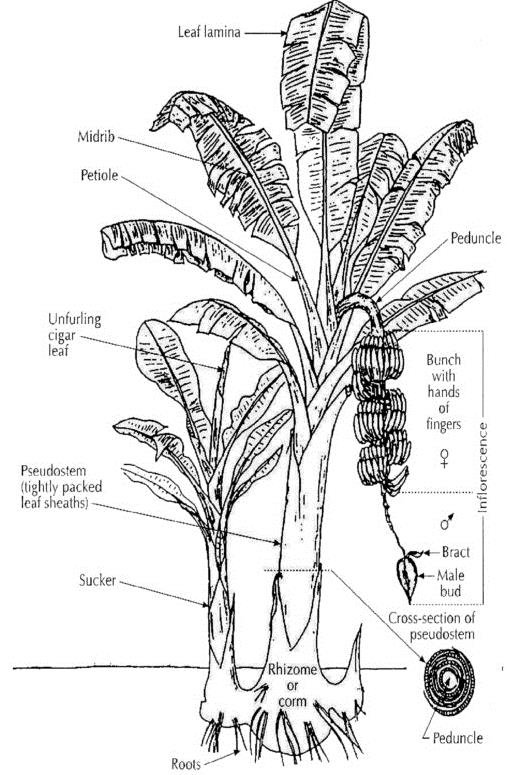
\includegraphics[width=12cm]{Figures/Diagrammatic-representation-of-a-fruiting-banana-plant-with-suckers-in-Bakry-et-al_W640.jpg}
    \caption[Anatomy of fruiting banana plant]{\textbf{Anatomy of fruiting banana plant}. From \textcite{Bakry2009}.}
    \label{fig:Anatomy of fruiting banana plant}
\end{figure}
\clearpage

\subsection{The History of Banana}

Originating from Southeast Asia, naturally occurring parthenocarpic – developing fruit without fertilisation – individuals of banana have been cultivated for about 10,000 years. Evidence of this can been seen in \textit{Musa banksii} phytoliths discovered in the Kuk swamp in Papua New Guinea \parencite{Denham2011}. Cultivated bananas were spread from Papua New Guinea, hybridising with subspecies of \textit{M. acuminata} and \textit{M. balbisiana} in the Philippines and northern New Guinea \parencite{Perrier2009}. Triploid cultivars were produced as a consequence and were dispersed throughout Southeast Asia, Northern Australia, East Africa, and South Asia by the Austronesian peoples, where, although primarily cultivated as a food crop, banana was also used in traditional medicine to treat ailments including dysentery, ulcers, leprosy, epilepsy, and insect bites \parencite{Kumar2012}. In these regions, banana has also been used as fodder; in domestic materials, such as plates, children’s toys, and dyes; in buildings for shelters, rafts, or rope; and has significant social and cultural value, involved in many traditional rituals and customs \parencite{Hapsari2017}.  

Banana cultivation continued to move into the Middle East and Northern Africa from the centre of domestication in Southeast Asia, which can be seen in references to banana in historic texts such as Ibn al-'Awwam's 12th-century agricultural work, \textit{Kit\=ab al-Fil\=a\d{h}a} (Arabic:\\ \<كتاب الفلاحة>, lit. \textit{Book of Agriculture}) \parencite{Clement1866}. Later, during expeditions in Southeast Asia and Africa in the mid-1500s, bananas were encountered by Europeans who transported plants to South America where colonists established banana plantations to supply the USA and Europe \parencite{Guzman-Rivas1960, Salas-Pascual2022}. This legacy continues today, with over 70\% of the EU’s banana supply coming from South American countries \parencite{EuropeanUnion2022}.  

\subsection{Cultivation and Value of Banana}
\label{sec:cultivation}

Global production now takes place year-round in tropical and subtropical regions where plants are commercially grown as a monoculture crop, although plants are also cultivated by smallholders and in subsistence production systems \parencite{Viljoen2020}. Commercially, fruits are harvested within about 9-12 months of planting (either\textit{ in vitro} propagated material or suckers) and are grown as a ratoon crop – the plant is cut back to the rhizome once the fruit has been harvested and left to regrow – for several years, by which time yields will have reduced and a new plantation must be generated. 

Today, banana is frequently reported as one of the world’s top agricultural commodities, the annual global production of bananas (including plantain) steadily increased from 98.4 million tonnes in 2000 to an estimated 155.2 million tonnes in 2018  and global exports increased from 15,540 tonnes in 2011 to 20,465 tonnes in 2021 \parencite{FAO2022}. Despite this, only around 15\% of bananas produced worldwide are traded in international markets. The remaining 85\% are consumed locally, highlighting the value of bananas as a subsistence crop, illustrated in developing countries where fruits can account for 25\% of daily calorie intake and act as a source of income \parencite{FAO2019}. The world’s largest banana growers are India and China which produced over 30 million tonnes and 11 million tonnes in 2021, respectively \parencite{BananaLink2023} (Figure ~\ref{fig:bananaProdMap}).  Currently, up to 40\% of all global banana production (domestic and export markets) is reliant on the Cavendish banana \parencite{Warman2018}, a triploid, clonally propagated subgroup deriving from \textit{M. acuminata}.

\begin{figure}[h!]
    \centering
    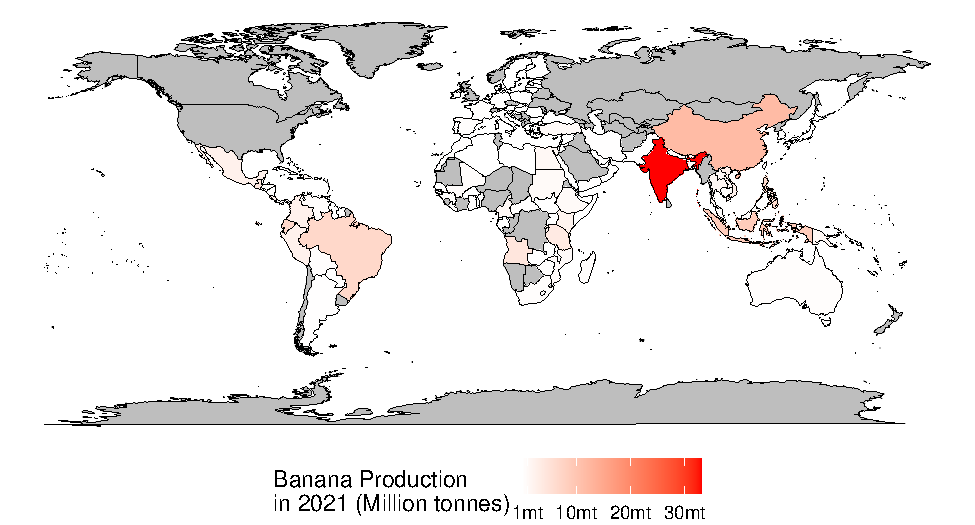
\includegraphics[width=\textwidth]{Figures/BananaProdMap.pdf}
    \caption[Global banana production, 2021]{\textbf{Global banana production (million tonnes), 2021.} No data available for countries in grey (Data source: BananaLink, 2023).}
    \label{fig:bananaProdMap}
\end{figure}

\section{Bananageddon: An Introduction to \acl{Focub}}
In recent decades, there have been reports of a potential ‘Bananageddon’, whereby global banana production is decimated by the fungal pathogen \acf{Focub} \acf{tr4}, the causative agent of \ac{fwb} (syn. Panama disease). The global banana community’s concern is demonstrated through the establishment of the \acs{tr4} Task Force, part of the \ac{FAO} \ac{wbf}; the Peruvian government’s declaration of a National Emergency upon the discovery of \ac{Focub4} in 2021 (FAO, 2021); and in the review by \textcite{Westerhoven2022}, where the authors stress \ac{Focub4}'s threat to African food security.   

\subsection{A Brief History of Fusarium Wilt}
\label{chap1:focHistory}
A robust response to \ac{Focub4} is not unfounded. During the first half of the 20th century, \ac{Focub1} devastated global production, destroying  ~40,000 hectares of ‘Gros Michel’ plantations \parencite{Agrios2005, Kema2021}, and resulted in estimated economic losses of \$400 million (USD) between 1940 and 1960 (equivalently to \$4.117 billion or £3.259 billion in 2023)\parencite{Ploetz2005}. \ac{Focub1} eventually led to the disappearance of ‘Gros Michel’ as an export banana in the 1960s \parencite{Molina2007}, when the \ac{Focub1} resistant Cavendish bananas subsequently replaced ‘Gros Michel’ \parencite{Ordonez2015a}. 

The threat posed by \ac{Focub} remains, however. In the 1960s Cavendish banana plants in Taiwan were observed displaying symptoms of \ac{Focub} infection \parencite{Agrios2005}. Identified in 1994 as \ac{Focub4} \parencite{Ploetz1994} the strain affecting Cavendish bananas has continued to spread. \Ac{Focub4} is now found in Africa, Asia, and Europe \parencite{Ploetz2015a, Thangavelu2019} and is gaining a foothold in South America, with recent incursions in Colombia in 2019 \parencite{Garcia-Bastidas2019}, Peru in 2021 \parencite{Acuna2022}, and Venezuela in 2023 \parencite{Herrera2023}.

\subsection{Disease Development of \acl{Focub}}

As a soil-borne pathogen, \ac{Focub} first colonises the roots. Asexual spores in the soil germinate in response to host root exudates and infection hyphae produced from resting spores (chlamydospores) penetrate the root epidermis at the tip \parencite{Li2011}. \ac{Focub} hyphae progress through the root cortex to the rhizome and migrate through the xylem in the outer leaf sheaths of the pseudostem, occluding vessels and interfering with nutrient uptake and upward water transport; often before visible symptoms are observed \parencite{Li2017, Warman2018}. 

Mycelia produce microconidia within the xylem vessels, and microconidia travel up through the transpiration stream \parencite{okungbowa2012fusarium}. Conidia and hyphae become 'trapped' at naturally occurring end walls or perforation plates of the xylem strands, which somewhat restricts pathogen movement through the host. \textcite{vandermolen1977vascular} observed that microconidia trapped at the perforation plates germinate and penetrate the plate, allowing the pathogen to continue to progress through the plant.

Xylem vessels begin to collapse, and external symptoms are observed. Tissues become chlorotic, and the plant withers as it transpires more than it can translocate. Once the plant dies, the fungus begins to invade other plant tissues and sporulate, particularly on the plant surface. \textcite{Warman2018} observed substantial production of macroconidia and chlamydospores attached to the outside of decaying root tips and formed in sporodochia on dead leaves, acting as secondary sources of inocula \parencite{ohara2004ren1} (Figure: \ref{fig:MyLifeCycle
}). Chlamydospores can persist in the soil for decades and are resistant to adverse conditions \parencite{Pegg2019}. 

Alternative hosts, including many grass and weed species, act as a reservoir of inoculum \parencite{Hennessy2005}.  \ac{Focub} is dispersed through the movement of contaminated plant and soil material, water, wind, and people. Typical symptoms of \ac{Focub} infection include discolouration and splitting of the pseudostem, yellowing of lower leaves often forming a ‘skirt’ around the plant, and a streaking pattern is occasionally observed on the foliage (Figure ~\ref{fig:FusariumWiltSymptoms}). 

\begin{figure}[p!]
    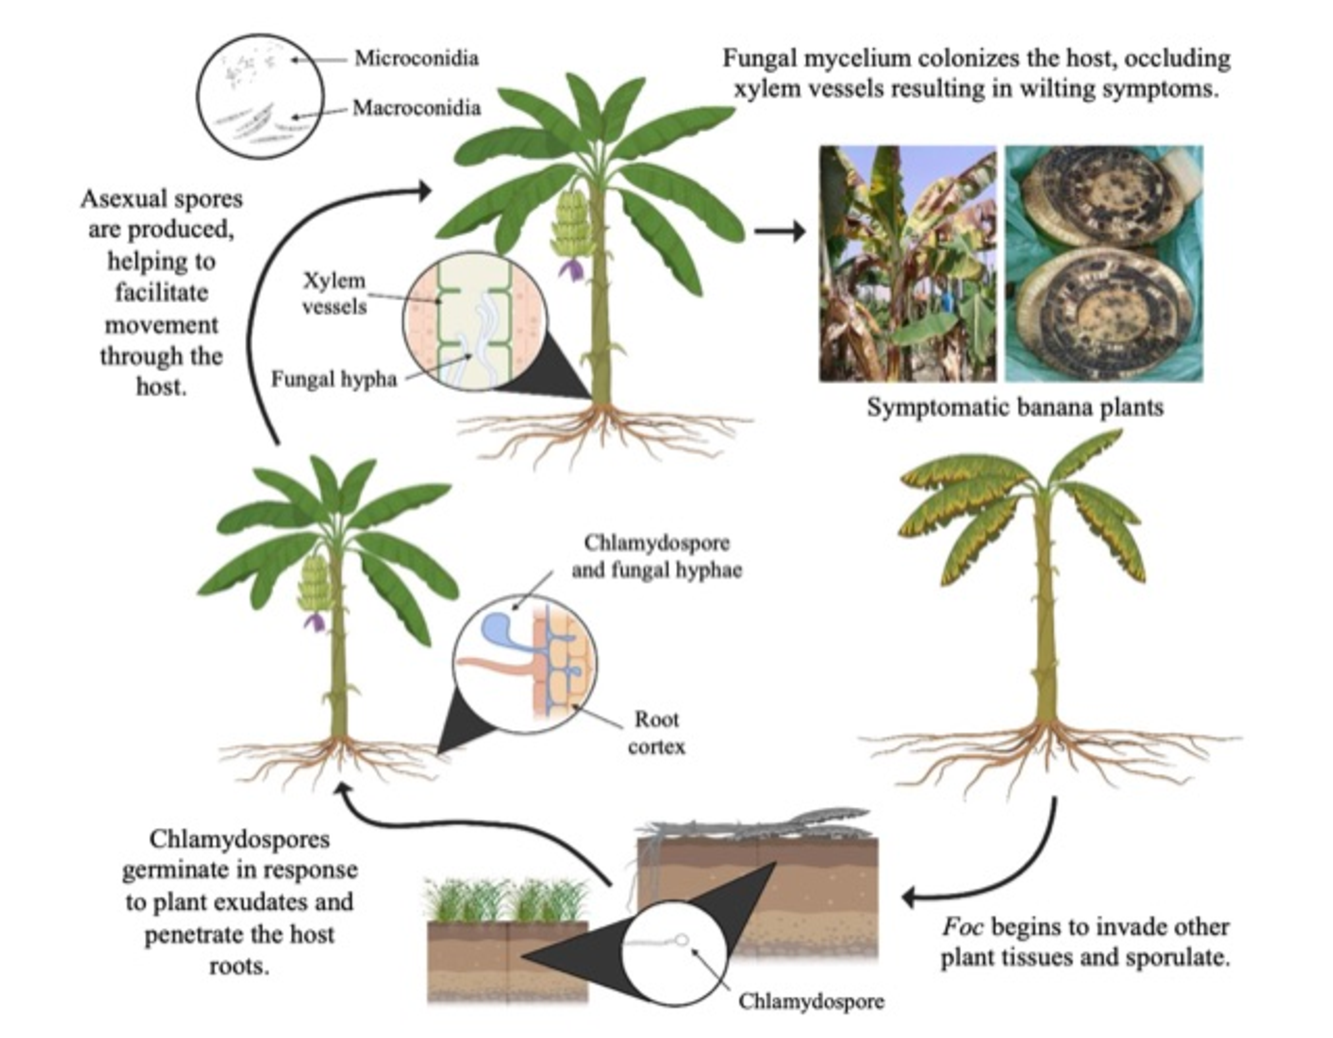
\includegraphics[width=16cm]{Figures/MyLifeCylceNarrow.pdf}
    \caption[Fusarium wilt of banana disease cycle.]{\textbf{Fusarium wilt of banana disease cycle.} Chlamydospores germinate in the soil in response to plant root exudates. Infection hyphae from chlamydospores penetrate the root tip epidermal cells and progress through the host root cortex to the xylem. Microconidia and macroconidia are produced in the xylem and help to facilitate pathogen movement through the host. As \acl{Focub} migrates through the xylem it occludes vessels and interferes with nutrient uptake and upward water transport. External wilting symptoms begin to develop; tissues become chlorotic and the plant withers as it transpires more than it can translocate. Eventually, the plant dies, and asexual spores are formed on the dead tissue. Chlamydospores persist in the soil or \acl{Focub}  survives endophytically in an alternative host species. Fungal hyphae are shown in blue. Images of \acl{Focub}  spores adapted from \textcite{Fourie2011} and symptomatic banana plant images sourced from \textcite{Maymon2020}. Figure created with BioRender.com.}
    \label{fig:MyLifeCycle}
\end{figure}

\begin{figure}[pt!]
    \centering
    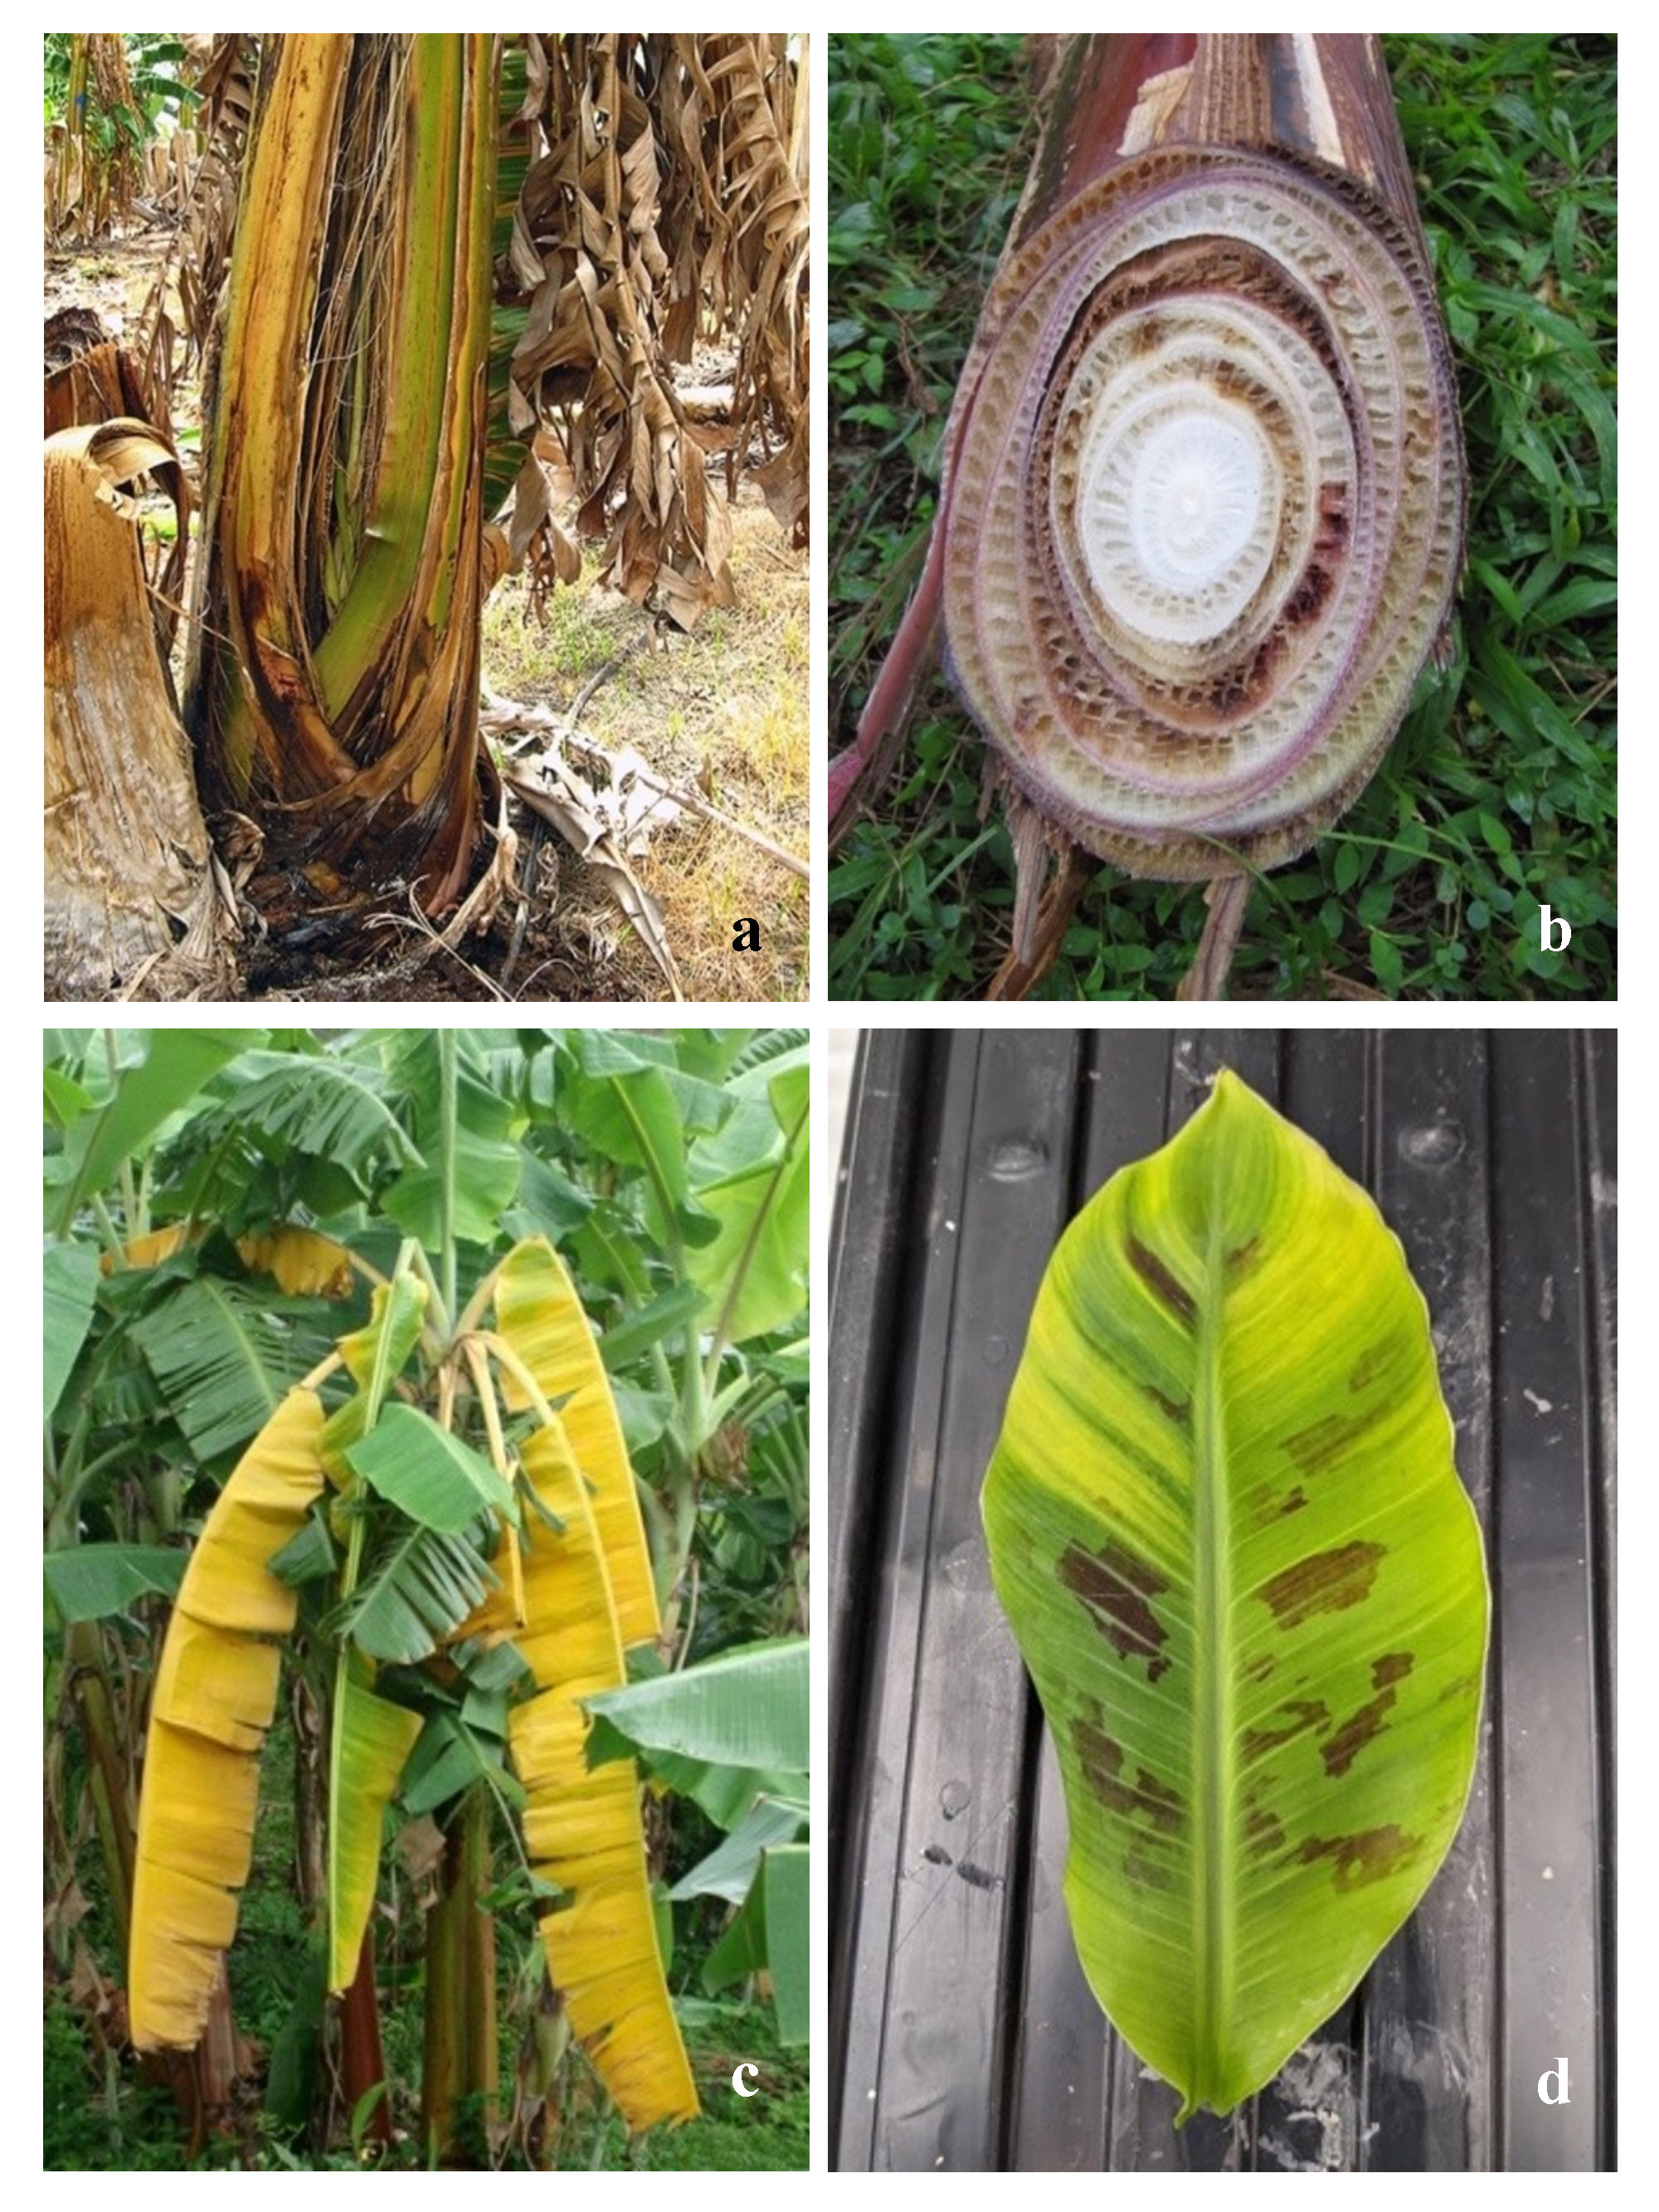
\includegraphics[width=15cm]{Figures/SymptomsofFoc.pdf}
    \caption[Typical symptoms of \textit{Fusarium}  wilt of banana.]{\textbf{Typical symptoms of \textit{Fusarium} wilt of banana.} (a) Splitting of the pseudostem, (b) discolouration of the pseudostem, (c) yellowing of lower leaves, and (d) streaking pattern is observed on the foliage. Photos by Dita, M (a) and Blomme, G (b and c), Bioversity International.}
    \label{fig:FusariumWiltSymptoms}
\end{figure}

\subsection{Classification of \acl{Focub}}

\ac{Focub} belongs to the \acf{FOSC}. The species complex contains both plant and animal pathogens, as well as saprophytes and endophytes \parencite{Leslie2006}. The \ac{FOSC} has high functional and genetic diversity, shown plainly in its broad plant host range. The species complex can infect around 150 species of both monocotyledonous and dicotyledonous plants, including many horticulturally important crops such as banana, tomato, and lettuce \parencite{Edel-Hermann2019}.  Individual pathogenic \ac{Fo} isolates can infect only one or a few plant species. Plant pathogenic \ac{Fo} are therefore divided into ‘special forms’, or \acfp{fsp}, each of which is adapted to specific hosts \parencite{Snyder1940}. For instance, strains which cause Fusarium wilt in tomato are classified as \acl{Foly}. To date, 106 \acp{fsp} have been clearly described, with at least an additional 37 putative \acp{fsp} \parencite{Edel-Hermann2019}.   

Some \acp{fsp} can be further subdivided into pathogenic races, determined by pathogenicity towards specific host cultivars. Three races of \ac{Focub} affecting banana have been identified. \acf{r1}  affects banana cultivars such as ‘Gros Michel’ (AAA), ‘Maqueno’, ‘Silk’, ‘Pome’ (AAB), and ‘Pisang Awak’ (ABB); \acf{r2} affects ‘Bluggoe’ and other cooking bananas (ABB); Race 4 affects the subgroup Cavendish (AAA) as well as hosts of \ac{r1} and \ac{r2} \parencite{Ploetz2015a} and has been further divided into \ac{str4} and \acl{tr4}. \Ac{tr4} is distinguished from \ac{str4} as it affects susceptible cultivars without disease-predisposing conditions \parencite{Ploetz2015b}.  

Classification of isolates based on race is often subjective. During the 1980s an additional method of \ac{Focub} identification based on \acf{vcg} was developed \parencite{Correll1991}. \acp{vcg} are comprised of isolates that possess the same alleles at all \ac{vic} loci, and so can form stable heterokaryons with each other \parencite{Correll1991}. So far, 24 \acp{vcg} of \ac{Focub} have been confirmed in \ac{Focub} (Table ~\ref{tab:VCGTab}) \parencite{Czislowski2018}, though \textcite{Mostert2022} have since reported additional \ac{Focub} \acp{vcg}. Some \acp{vcg} of \ac{Focub} are taxonomically closer to other \acp{fsp} of \ac{Fo} than other \ac{Focub} \acp{vcg}. This, coupled with distinct genetic lineages identified through phylogenetic analysis, has resulted in the recognition of a polyphyletic – taxonomic group including members from different ancestral lineages – evolutionary history for \ac{Focub} \parencite{Koenig1997, Ploetz2007}. 

\textcite{Maryani2019} revised the taxonomy of \ac{Focub}, generating the Fusarium of Banana Species Complex and proposing several new species. However, \textcite{Torres2021} have suggested that the revision is premature and that the data do not fully support the revision. There continues to be active debate surrounding \ac{Focub} classification and a clear, robust, universally accepted taxonomy has not yet been established. Race, although somewhat informal, remains the most widely accepted method of \ac{Focub} classification – whereby isolates are identified based on virulence towards specific host cultivars.  

\afterpage{

%Insert the VCG table
% Please add the following required packages to your document preamble:
% \usepackage{longtable}
% Note: It may be necessary to compile the document several times to get a multi-page table to line up properly
\begingroup
\setlength{\tabcolsep}{28pt} % Default value: 6pt
\renewcommand{\arraystretch}{0.75}
\begin{longtable}[tc!]{ccc}
\caption[\acf{vcg} of \ac{Focub}]{{\textbf{\acf{vcg} of \ac{Focub}} and race (Czislowski \et 2018).} Cross-compatible VCGs can form VCG complexes.}
\label{tab:VCGTab}\\
\hline
\textbf{VCG} & \textbf{VCG   complex} & \textbf{Race}    \\ \hline
\endfirsthead
%
\multicolumn{3}{c}%
{{\bfseries Table \thetable\ continued from previous page}} \\
\endhead
%
0120  & 0120–01215           & STR4             \\
0121  &                      & R4               \\
0122  &                      & R4               \\
0123  &                      & R1               \\
0124  & 0124–0125–0128–01220 & R1,   R2         \\
0125  & 0124–0125–0128–01220 & R1, R2           \\
0126  &                      & R1               \\
0127  & No longer valid      & No longer valid  \\
0128  & 0124–0125–0128–01220 & R1,   R2         \\
0129  & 0129–01211           & STR4             \\
01210 &                      & R1               \\
01211 & 0129–01211           & STR4             \\
01212 &                      & Not   Identified \\
01213 & 01213–01216          & TR4              \\
01214 &                      & R2               \\
01215 & 0120–01215           & STR4             \\
01216 & 01213–01216          & TR4              \\
01217 &                      & R1               \\
01218 &                      & R1               \\
01219 &                      & Not identified   \\
01220 & 0124–0125–0128–01220 & R1               \\
01221 &                      & Not Identified   \\
01222 &                      & Not   Identified \\
01223 &                      & Not Identified   \\
01224 &                      & Not   Identified \\ \hline
\end{longtable}
\endgroup

\clearpage
}

\subsection{The \acl{Fo} genome} 

An emerging explanation for host specificity in different \acf{Fo} lineages relates to the compartmentalisation of the \ac{Fo} genome, a theory that has become increasingly prevalent in \ac{Fo} genomics following the work of \textcite{Ma2010}. This study explains that the \textit{Fusarium} genome can be organised into two parts containing either \acp{cc} or \acp{ac} (syn. pathogenicity/lineage-specific/supern\-umerary chromosomes). The 11 \acp{cc} within the \ac{Fo} genome encode functions necessary for primary metabolism and reproduction \parencite{Dam2017}. The remaining \acp{ac}, which vary in number among \acp{fsp}, are not required for primary metabolism and reproduction, contain secondary metabolite biosynthetic gene clusters, encode virulence genes such as effectors, and possess a high number of \acp{te} \parencite{Ma2010, Schmidt2013, Witte2021}. Further, \textcite{Ma2010} suggests these \acp{ac} can be horizontally transferred and afford host-specific pathogenicity to the recipient. A theory which has since been demonstrated in \acf{Foly} \parencite{Vlaardingerbroek2016a, Vlaardingerbroek2016b, Li2020a}, \ac{Fo} f. sp. \textit{radicis-cucumerinum} \parencite{Dam2017} and \ac{Fo} f. sp.  \textit{melonis} \parencite{Li2020b}. 
 
Not only do \acp{ac} go some way to explaining diversity between \acp{fsp}, but also among strains within specific \ac{fsp}. For instance, a recent preprint by \textcite{Westerhoven2023} analyses the dynamics of \acp{ac} in \ac{Focub} and explores the role segmental duplications have in \ac{ac} evolution and diversity within \ac{Focub}. \textcite{Westerhoven2023} sequenced and assembled 69 \ac{Focub} strains (including \ac{r1}, \ac{r2}, and \ac{tr4})  isolated from various banana-growing regions. They generated chromosome-level genome assemblies and identified \acp{ac} in these strains.  The authors reported a significant amount of variability of the \acp{ac} between the \ac{fwb} strains, for instance, \acp{ac} ranged in size from 6.7Mb to 16.5Mb and exhibited extensive diversity in gene content, repeat content, and GC content when compared to the \ac{Focub} core chromosomes. \Acp{ac} are most commonly shared among strains of \ac{Focub1} from the same lineages, and few \acp{ac} are shared between \ac{r1} lineages. \Acp{ac} in \ac{Focub4} strains, however, showed low nucleotide diversity and the authors suggest that \ac{Focub4} evolved from a single recent clonal origin. 

The manuscript by \textcite{Westerhoven2023} highlights the prevalence of segmental duplication in \acp{ac} and sub-telomeric regions of \ac{Focub}. The authors demonstrate that these duplications are associated with the recent evolution and diversification of genes, including virulence genes, and play a crucial role in the expansion and adaptation of \acp{ac} in the \ac{FOSC} genome. However, it is worth noting that this manuscript has not currently published (February 2024) the \ac{Focub} assemblies generated, nor does it provide an appropriate data set detailing the assembly quality of the isolates sequenced for the study, making it challenging to validate the authors' conclusions. 

\subsection{The Plant Innate Immune System}

As a plant pathogen, \ac{Fo} faces considerable evolutionary pressure to develop diverse mechanisms that can evade host detection and facilitate successful infection. The wide diversity of \acp{ac}, their ability to function separately from \ac{Fo}'s \ac{cc}, and the high number of \acp{te}  suggests that this specific section of the genome serves to fulfil the pathogen's adaptive needs in its interaction with hosts and evade plant defence mechanisms.

Plants have coordinated defence mechanisms which enable them to detect and respond to invading pathogens effectively. The plant’s innate immune system is comprised of two interconnected tiers which perceive and respond to pathogen infection \parencite{Jones2006, Han2019, DeFalco2021}. The first tier recognises microbial- or \ac{pamp} which are slow-evolving, conserved molecules (such as the fungal cell wall component, chitin) using transmembrane \ac{prr} on the plant cell surface. Once \ac{pamp} have been recognised, \ac{pti} is induced, including numerous cell signalling events such as altered ion fluxes, the production of apoplastic reactive oxygen species, callose deposition, and transcriptional reprogramming. 

To evade, suppress, or interfere with \ac{pti} responses and establish infection, fungal pathogens secrete proteins termed ‘effectors’ into the host cell which results in \ac{ets}. To combat \ac{ets}, plants possess a suite of \ac{rprot} which perceive effectors (termed '\ac{AVR} proteins') and induce further immune responses, known collectively as \ac{eti} \parencite{Jones2006} (Figure:~\ref{fig:PlantImmuneSystem}). \Ac{rprot} are conserved intracellular receptors of the \ac{nlr} class. The structure, function, and effector perception (direct or indirect) of \ac{rprot} is variable and often specific  \parencite{Chen2022, Wang2022}. Similarly, effectors are typically highly variable and specific to individual pathogens \parencite{LoPresti2015}. \textcite{Gutierrez2023} have prepared a comprehensive review of virulence factors in the \textit{Fusarium} genus. 

\begin{figure}[h!]
    \centering
    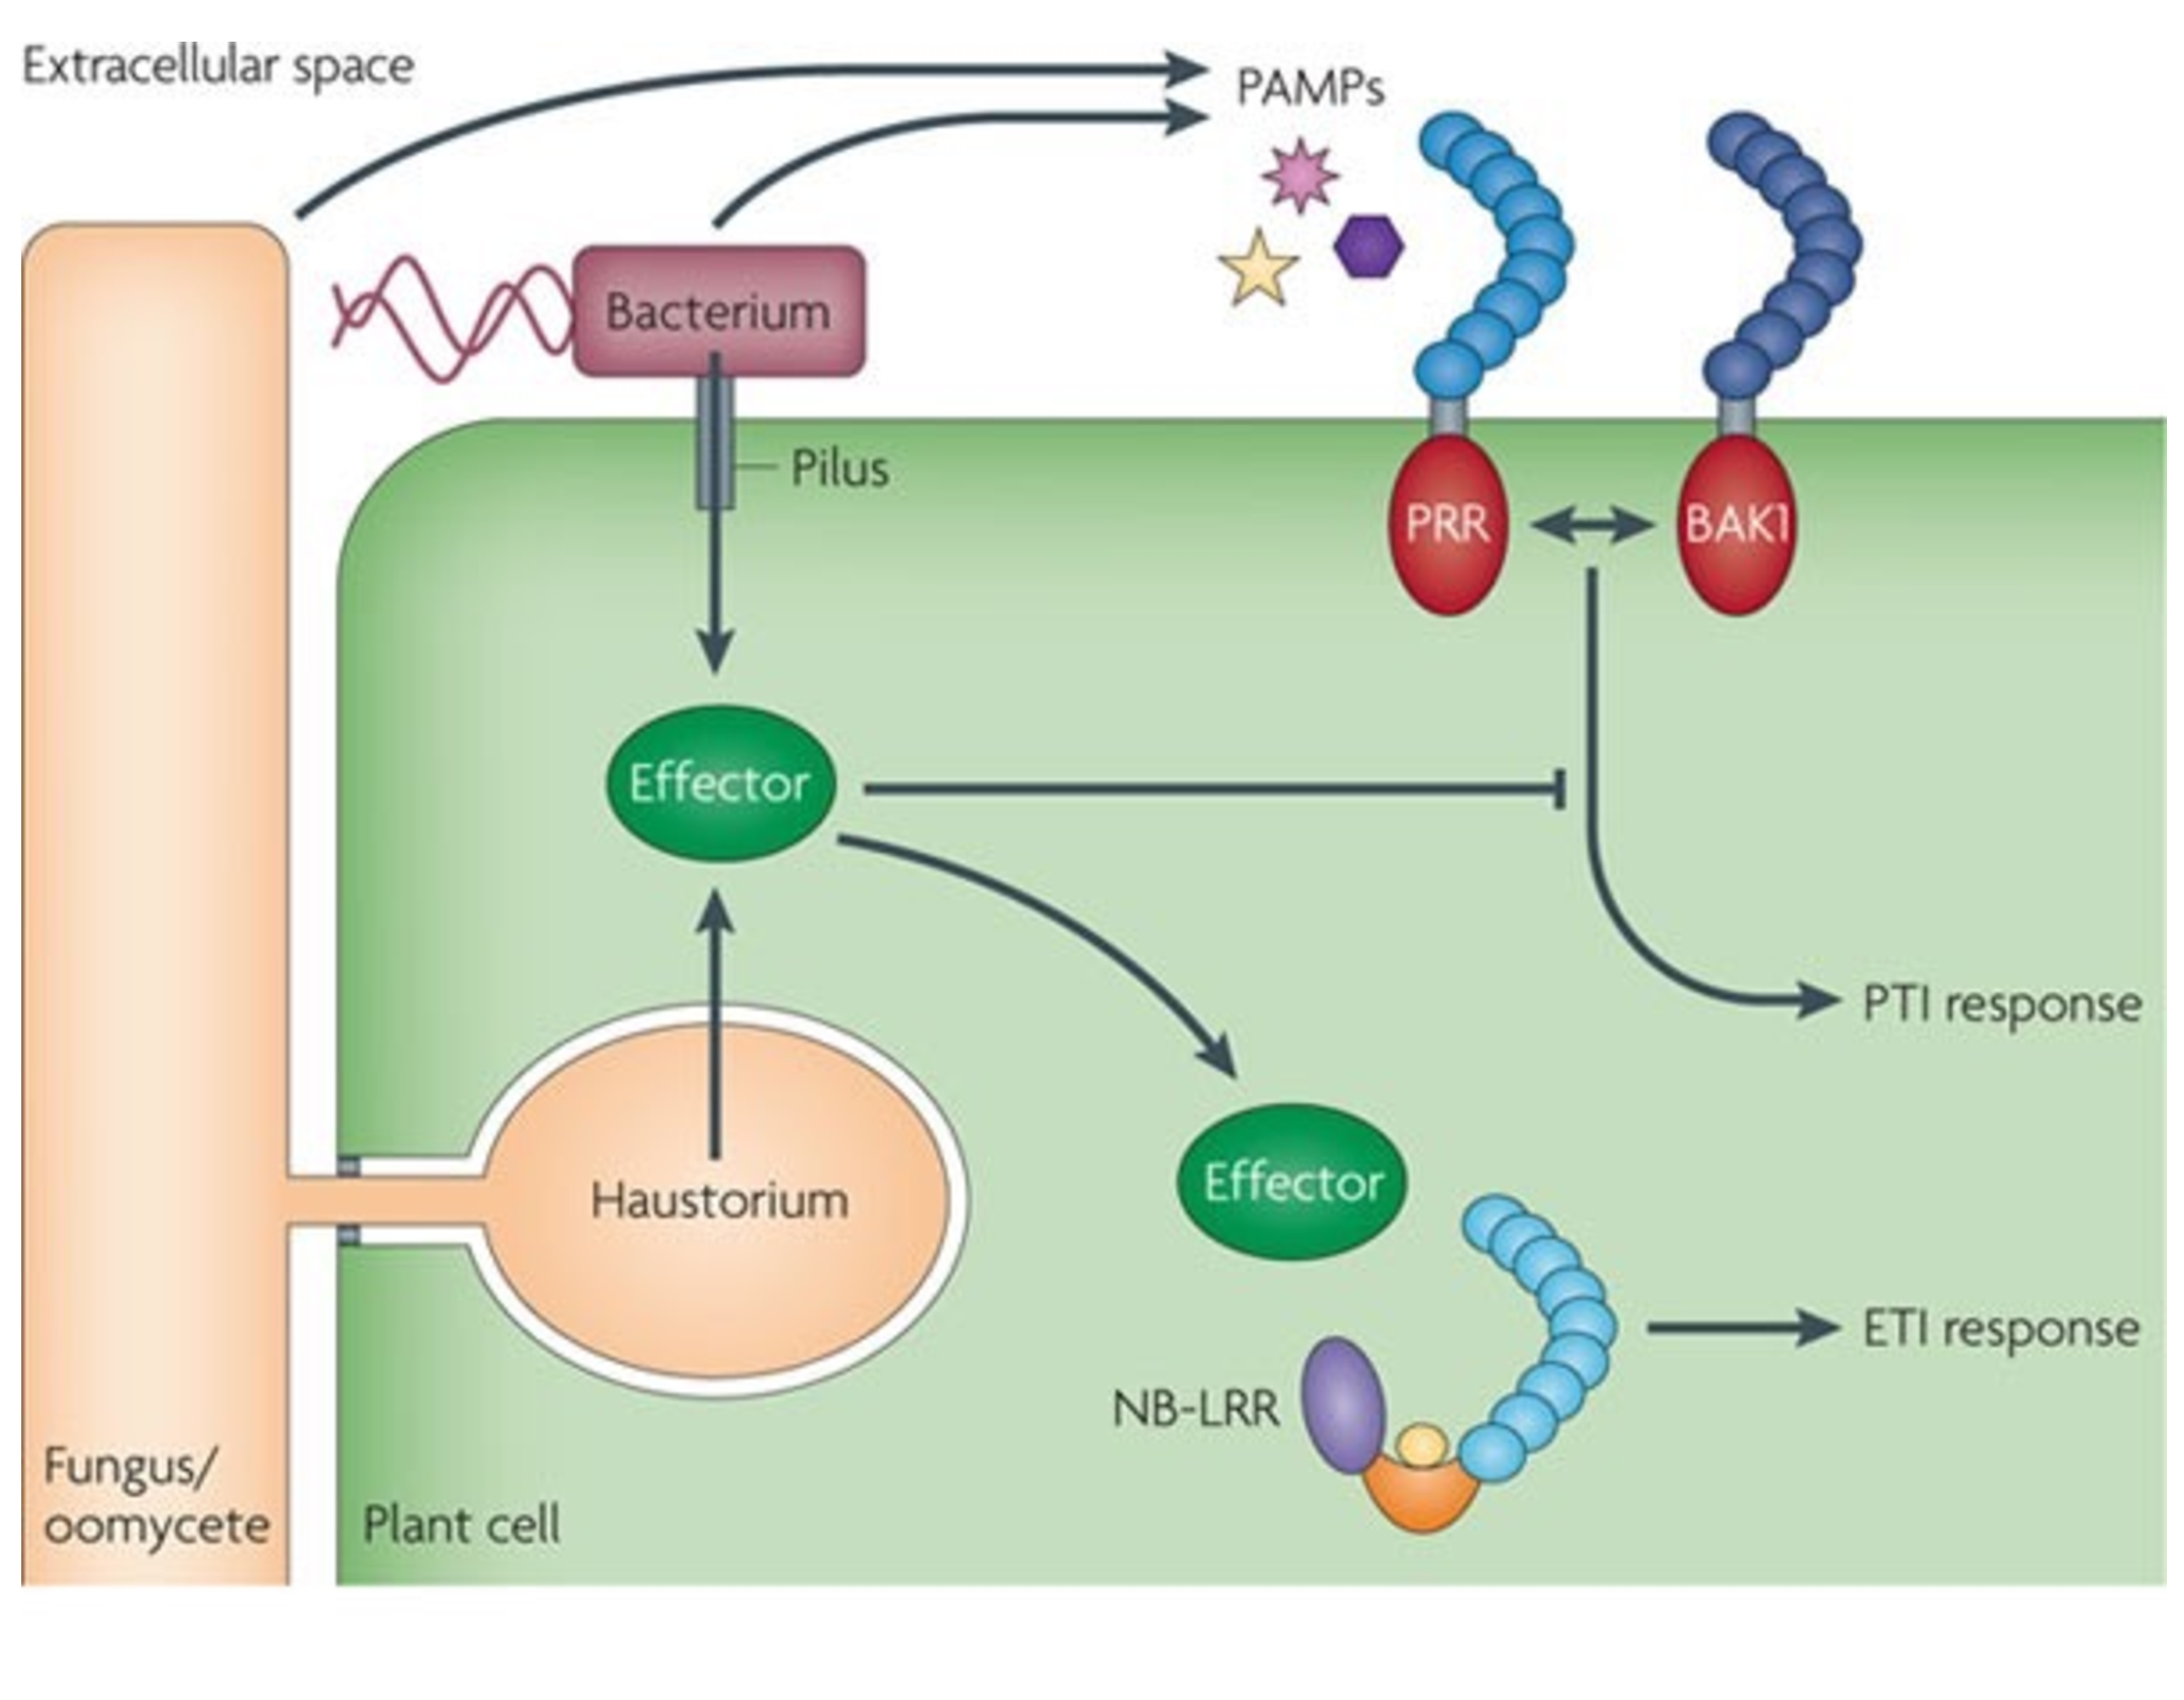
\includegraphics[width=\textwidth]{Figures/DoddsArticleModel.pdf}
    \caption[Overview of the plant immune system.]{\textbf{Overview of the plant immune system.} Pattern recognition receptors (PRRs) perceive microbial- pathogen-associated molecular patterns (MAMPs/PAMPs) and induce a PAMP-triggered immunity (PTI) response from the host. To overcome host cell defences, pathogens secrete small molecules known as effectors into the host cell, inducing effector-triggered susceptibility (ETS). Plants have adapted a family of resistance proteins (R proteins), which can perceive pathogen effectors (avirulence proteins) and stimulate an effector-triggered immunity (ETI) response from the plant host (From Dodds and Rathjen, 2010).}
    \label{fig:PlantImmuneSystem}
\end{figure}


\subsection{The \acl{Fo} Effectorome}
\label{Chap1:fusariumEffectorome}

In the \ac{FOSC}, the only family of effectors currently recognised are the \acfp{sixg}. In total, 14 SIX proteins (SIX1 – SIX14) have been identified through mass spectrometry of infected tomato xylem sap and whole genome sequencing \parencite{Houterman2007}.  All 14 \acp{sixg} are found on the \acp{ac} in \ac{Foly} \parencite{Schmidt2013}, and studies have confirmed that \textit{SIX1, SIX2, SIX3, SIX5}, and \textit{SIX6} are essential for conferring virulence in tomato, with  \textit{SIX4} (\textit{Avr1}), \textit{SIX3} (\textit{Avr2}), and \textit{SIX1} (\textit{Avr3}) all recognised by corresponding \ac{rprot} (called ‘I-’ for Immunity) in tomato \parencite{Rep2004, Lievens2009, Takken2010, Gawehns2014, Ma2015}. 

The function of most \acp{sixg} is not yet known \parencite{Czislowski2018, An2019, jobe2024secreted, daniel2024structural}, however, potential functions have been explored for some \acp{sixg}. In \textit{F. oxysporum} f. sp. \textit{conglutinans}, SIX8 and Pair with SIX Eight1 (PSE1) are a divergently transcribed effector gene pair that function together to suppress phytoalexin production and plant immunity in \textit{Arabidopsis} \parencite{ayukawa2021pair}. SIX3 and SIX5 have been shown to as act as an effector pair that interacts with the plasmodesmata, with \textcite{cao2018fusarium} showing that the effector pair facilitates the movement of SIX3 to neighbouring cells. \textcite{blekemolen2022primary} later observed that the SIX3/SIX5 effector pair facilitates the movement of two further effectors, SIX6 and SIX8, to neighbouring cells however, the mechanism the SIX3/SIX5 effector pair employs to manipulate the size exclusion limit of plasmodesmata and facilitate cell to cell movement of effectors remains unknown \parencite{blekemolen2022primary}. 

As well as operating in the SIX3/SIX5 effector pair, SIX3 interacts with BOTRYTIS-INDUCED KINASE 1 (BIK1) in \textit{Arabidopisis thaliana} \parencite{blekemolen2023pti}. BIK1, a downstream signalling kinase of the \acf{prr} co-receptor, BRI1-ASS\-OCIATED RECEPTOR KINASE (BAK1). \textcite{blekemolen2023pti} observed SIX3 and BIK1 co-localise \textit{in planta}, that SIX3 affected BIK1 abundance, shifted BIK1 localisation from nucleocytoplasmic regions to the cell periphery/plasma membrane, and that SIX3 compromised mono-ubiquitination of BIK1. \textcite{blekemolen2023pti} therefore suggested that SIX3 retains BIK1 at plasma membrane and suppresses the ability of BIK1 to activate immune signalling, with the interference with mono-ubiquitination of BIK1 by SIX3 serving as a potential mechanistic explanation. 

Since their discovery in \ac{Foly}, homologs of \acp{sixg} have been identified in other \acp{fsp}, including \textit{cepae, conglutinans, fragariae, melonis, pisi, radicis-cucumerinum,} and \textit{vasinfectum} \parencite{Czislowski2018}. A further \textit{SIX} gene, (\textit{SIX15}) has been described by \textcite{Simbaqueba2018} in \acl{Fo} f. sp. \textit{physalis}, although \textit{SIX15} is not widely reported. 

In \ac{Focub}, homologs of \textit{SIX1, SIX2, SIX4, SIX6, SIX7, SIX8, SIX9}, and \textit{SIX13} have been identified, and \textit{SIX1} and \textit{SIX8} have been recognised in \ac{Focub} \ac{tr4} as essential for virulence through knockout mutants \parencite{Widinugraheni2018, An2019}. Interestingly, \textcite{Fraser-smith2014} observed differences in \textit{SIX8} sequence between \ac{tr4}, \ac{str4}. \textcite{Czislowski2018} reported differences in the \ac{sixg} repertoire of \ac{Focub} \ac{r1} and \ac{r4} lineages and hypothesised that the differences in \ac{sixg} profiles contribute to the variability in the \ac{Focub} host cultivar range.  However, as suggested, \acp{sixg} are unlikely to be the only set of effectors involved in host specificity, and  \textcite{Czislowski2018} state "it should be expected that novel and undiscovered effectors remain to be identified in the lineages of \ac{Focub}".  

\textcite{Ma2010} showed that the \acp{ac} in \ac{Foly}, have a high number of retro-elements, including the non-autonomous class II \acf{te}, \ac{mites}. A specific family of \ac{mites}, known as \acfp{mimp}, are found upstream of all known \acp{sixg} in \ac{Foly} \parencite{Schmidt2013}. Characterised by their \ac{tir} sequence and short length ($\sim$180–220 \acs{bp}), \textcite{Schmidt2013} surmised that \acp{mimp} could be used for the prediction of effectors in \ac{Fo}, particularly \acp{sixg}, a theory later demonstrated by \textcite{Dam2016, Dam2017, Armitage2018, FoEC2}.  

The hypothesis that effector profiles contribute to host specificity is proposed for other \ac{fsp} \parencite{Achari2021, Batson2021} and is tested on the host species level for the \ac{FOSC} \parencite{Dam2016}. With advances in genome sequencing and analysis, it is possible to identify new candidate effectors using common characteristics shared between known effectors in \ac{Foly} and other \ac{fsp}, as well as their location in the \ac{Fo} genome and evolutionary relationship.

\subsection{Control of \acl{Focub}}

There are few effective controls for \ac{Focub} in the wider environment. Chlamydospores can persist in the soil for decades and \ac{Focub} can invade non-host plants and survive as an endophyte, with grass and weed species acting as sources of inoculum \parencite{Pegg2019}. Biological control agents and fungicides have been investigated as a means of \ac{Focub} control. However, most of these are \textit{in vitro} and greenhouse assays which, although successful, are not practical or effective in-field \parencite{Dita2018}.  

As most commercial bananas are triploid and parthenocarpic, conventional breeding for resistance is exceedingly challenging \parencite{Dale2017}. One somaclonal variant of Cavendish, ‘Formosana’, is marketed as being resistant to \ac{tr4}. \textcite{wang2017differential} analysed differentially expressed genes in roots of ‘Formosana’ and the susceptible ‘Brazil’ banana plants infected with \ac{Focub4}. The authors identified 107 differentially expressed genes, 48 of which had known functions. Of the 48 genes, 41 were more highly expressed in ‘Formosana’. The 41 highly expressed genes were divided by the authors into several categories, including specific resistance mechanism-related enzyme genes and phytoalexin synthesis-related genes. The authors suggest that ‘Formosana’ may enhance its tolerance to \ac{Focub4} by increasing the expression of defence-related genes (possibly constitutively). \textcite{wang2017differential} also showed that ‘Formosana’ exhibits up-regulated expression of non-specific stress-related genes, and explained this may enhance the overall disease resistance in ‘Formosana’. Though tolerant to \ac{Focub4}, yields are slightly reduced in ‘Formosana’ due to its longer growth cycle and there have been reports of  ‘Formosana’ showing \ac{tr4} susceptibility in later field trials \parencite{Lee2011, Dale2017}. 

Another somaclonal variant, ‘Guijiao 9’, is also marketed as having lower disease severity compared to conventional commercial Cavendish varieties such as ‘Williams’ \parencite{Sun2019}. Similar to the study by \textcite{wang2017differential}, \textcite{Sun2019} conducted a comparative transcriptomic analysis of \ac{Focub4}-infected ‘Guijiao 9’, comparing gene expression to the \ac{Focub4}-susceptible ‘Williams’. The authors identified a "more drastic" response in ‘Guijiao 9’ to \ac{Focub4} infection compared to ‘Williams’, with genes associated with defence-related metabolite synthesis being significantly up-regulated in ‘Guijiao 9’. While ‘Guijiao 9’ presents a potential commercial solution for \ac{Focub4}, it has only recently been released to the market, and field trials outside the region in which this variety was developed have not yet been conducted.

Advances in genetic modification technologies have facilitated the development of two \ac{tr4}-resistant transgenic Cavendish lines \parencite{Dale2017}. One of these lines, ‘QCAV-4’ has just received regulatory approval in Australia \parencite{GMApproval}. The transgenic 'QCAV-4' variety was generated by transforming \textit{M. acuminata }Cavendish cv. 'Grand Naine' (AAA subgroup) embryogenic cell suspensions (prepared from immature male flowers) using the centrifugation assisted \textit{Agrobacterium tumefaciens}-mediated method with \ac{rga2}. \ac{rga2} is a putative \ac{nlr}-type \acl{rgene} from a seedling of \textit{M. acuminata} ssp. \textit{malaccensis} with resistance to \ac{Focub4}. However, the market for genetically modified crops within Europe is limited, although debate and legislation are currently under review and development. 

Gene-edited banana may be a more marketable alternative, particularly for Europe, and editing for disease resistance has been demonstrated in banana. \textcite{Tripathi2021} used CRISPR-Cas9 to make mutations to the downy mildew resistance 6 (DMR6) orthologue in banana, showing enhanced resistance to the bacterial pathogen \acf{xvm}, this approach may be applied to target a gene which could provide resistance to \ac{Focub}.  

\section{Bananomics: Tools and Technologies to Identify \textit{Fusarium} Wilt of Banana}
\label{sec:chap1-diagnostics}

Prevention of \ac{Focub} introduction has so far proven the most effective method of \ac{Focub} control on a large scale \parencite{Ploetz2015b}, with management primarily focused on hygiene practices and prevention. The development of accessible, fast, and accurate diagnostic tools is imperative. Molecular and image-based diagnostics have both been developed to identify \ac{Focub}. However, many of the current image-based diagnostics are unable to distinguish \ac{Focub} from other banana wilt pathogens, and the molecular assays struggle to accurately identify pathogenic races.  

\subsection{Molecular Diagnostic Approaches}
\Ac{pcr}-based methods of identification are routinely employed in the detection of \ac{Focub}, alongside \ac{vcg} screening and race typing. Assays have been developed by \textcite{Lin2009, Dita2010, Li2013a, Li2013b}. A study by \textcite{Magdama2019} reviewed the efficacy of these \ac{pcr}-based detection methods for the identification of \ac{Focub4} against 302 \textit{Fusarium} isolates, including 292 \ac{Fo} isolates. The authors demonstrated that the primers developed by \textcite{Lin2009, Li2013a} for \ac{str4} and \ac{tr4} identification displayed false positives for \ac{Focub} \ac{r1} and \ac{r2} as well as five non-pathogenic \ac{Fo} endophytes. Similarly, primers developed by \textcite{Dita2010} showed false positives for \ac{Fo} endophytes. 

\textcite{Magdama2019} concluded that the most effective primers for \ac{tr4} identification are those developed by \textcite {Li2013b} and that, due to the diversity of the \ac{FOSC}, a wider range of \ac{Fo} isolates should be assessed when developing assays, and that primer design should focus on a genetic locus related to virulence to limit false positives.  Indeed, the gene targeted for diagnostics by \textcite {Li2013b} was implicated in virulence as a result of a T-DNA insertion conferring reduced virulence. However, to date there has been no further characterisation of the gene by deletion, editing, or complementation to confirm its function. An initial search of the sequence (GenBank Accession: JX090598), which corresponds to the gene used by \textcite{Li2013b}, was therefore conducted using the BLASTN suite (\href{https://blast.ncbi.nlm.nih.gov/Blast.cgi?PAGE=MegaBlast&PROGRAM=blastn&PAGE_TYPE=BlastSearch&BLAST_SPEC=}{https://blast.ncbi.nlm.nih.gov/}) (nr database). Hits were for hypothetical proteins or putative pathogenicity proteins, many of which were based on the initial entry, JX090598. As a result, the predicted protein sequence was searched using InterProScan (\href{https://www.ebi.ac.uk/interpro/search/sequence/}{https://www.ebi.ac.uk/inter\-pro/search/sequence/}) (InterPro protein signature databases). InterProScan predicted a signal peptide in the first 1-25 aa, characteristic of fungal effectors. This, taken together with the target gene's small size (104 aa) and implied role in virulence, suggests it may be a fungal effector. As \textcite {Li2013b} and \textcite{Magdama2019} state that the diagnostic developed using the target gene identified by \textcite {Li2013b} is specific to \ac{Focub4}, this gene may be a fungal effector specific to \ac{Focub4}. Using the wealth of genomic data currently being generated for \ac{Fo}, further virulence genes could be identified without time-consuming screening assays, such as the TDNA insertional mutagenesis screen conducted by \textcite {Li2013b} and used as a target for race-specific diagnostics. 


\textcite{Ordonez2019} used genome data and Diversity Array Technology sequencing to identify new genomic markers for \ac{Focub4} identification and develop a \ac{lamp} assay for in-field \ac{Focub4} diagnostics. The \ac{lamp} primers were assessed for specificity against 67 isolates, including 22 \ac{tr4} isolates, 28 alternative \ac{Focub} \acp{vcg}, 16 other \ac{Fo} \ac{fsp} isolates, and one \textit{Ralstonia solanacearum} isolate. Although thorough, \textcite{Ordonez2019}  did not survey as many isolates as \textcite{Magdama2019}. Further research is required to determine if the sequences identified adhere to the recommendations of \textcite{Magdama2019}. 

\subsubsection{Effectors as a Target for \acl{Focub} Diagnostics}

Ideally, to develop molecular diagnostics that successfully distinguish between various \ac{Focub} races, \ac{Fo} \ac{fsp}, and endophytes, a key genetic locus with an important role in host-specific pathogen virulence should be targeted. \textcite{Dam2016,constantin2021number} demonstrated that \ac{Fo} possess different effector profiles, with a set of host-specific effectors depending on their target species and lifestyle.  

\textcite{Magdama2019} highlighted the importance of targeting specific genes for accurate diagnostics. Following this, diagnostic assays using \ac{pcr}-based methods targeting \acp{sixg} in \ac{Focub} have been developed by \textcite{Carvalhais2019}. These assays include simplex and duplex \acp{pcr} with additional restriction digestion steps. Primers specifically amplify regions of \textit{SIX6} in \ac{r1}, \textit{SIX1} in \ac{tr4}, \textit{SIX8} in \ac{str4}, \textit{SIX9/SIX10} in \ac{Focub} \ac{vcg} 0121 (R4), and \textit{SIX13} in \ac{Focub} \ac{vcg} 0122 (R4). The assays were validated using 250 \textit{Fusarium} isolates, including 16 different plant-associated \textit{Fusarium} species and 21 \acp{vcg}  commonly associated with \ac{Focub}. Amplicons were not generated for 5 of the 65 \ac{Focub} \ac{r1} isolates and the assay for \ac{Focub} \ac{vcg} 0121 generated false positives for three out of the 32 \ac{tr4} isolates. Furthermore, no known \ac{Focub} \ac{r2} isolates were used when validating the assays. Although effective in identifying isolates within \ac{Focub} R4, these assays arguably lack specificity for effective, accurate diagnostics of \ac{Focub} \ac{r1}, and specific groups within \ac{Focub} R4, and may provide false positives should an \ac{Focub} \ac{r2} isolate be sampled. This study indicates that \acp{sixg} provide a potential target for \ac{Focub} diagnostics, and access to a greater number of \ac{Focub} genomes may allow for more accurate primer development.  

\textcite{Chang2020} identified putative effectors as targets for diagnostics in \ac{Focub} using a \ac{mimp}-based approach. They identified candidate effectors in \ac{Focub} by searching local genome databases of \ac{Focub1} and \textit{Focub} R4 using 13 \ac{mimp} sequences from \textcite{Dam2016}. They identified 20 candidate effectors; 3 unique to \ac{Focub1}, 6 unique to \textit{Focub} R4. To demonstrate the accuracy of their identification method, they generated a knockout mutant and its complement of one candidate effector, gene \textit{Foc 1324}. Virulence tests on banana plants demonstrated that \textit{Foc 1324} was a virulence factor required for the pathogenicity of \textit{Focub} R4. Confirmation of function is still required for all candidate effectors in this study. Furthermore, candidate effectors were only identified in two genomes, one \ac{r1} genome and one R4 genome, \acp{vcg} for these genomes are not provided. Candidate effectors which \textcite{Chang2020} report are unique to \ac{r1} and R4 require further validation using more genomes representing different \ac{Focub} races.

Interestingly, the 13 mimp sequences identified by \textcite{Dam2016} in \ac{Focub} were found across three isolates, a considerably lower number of \acp{mimp} compared to other \acp{fsp} in their study. Our investigations revealed that the method of \ac{mimp} identification employed by \textcite{Dam2016} was flawed, being case sensitive (only searched for capitalised \ac{mimp} \acp{tir})\footnote{We made the authors aware, and they have subsequently updated their tool. See \textcite{FoEC2} }. Two of the \ac{Focub} genomes (B2 and N2) used had been repeat masked, therefore many potential \acp{mimp} in \ac{Focub} are likely to have been missed. A greater number of \ac{mimp}-associated effectors could have been discovered by \textcite{Chang2020} should they have had a query set of \ac{mimp} sequences more representative of those in \ac{Focub}.

In summary, leveraging the specificity of host-specific effectors in diagnostic assays could enhance the accuracy of detecting various \ac{Focub} races and distinguishing them from other \ac{Fo} \ac{fsp}, and endophytes. However, effective methods for host-specific effector identification must be developed in order for diagnostics to be developed. Access to a broader range of \ac{Fo} genomes and improving \ac{mimp} identification methods will likely result in more effective and precise diagnostic tools.

%\subsection{Image-based Approaches for Disease Diagnosis in Banana}
 
 %Non-invasive technologies, such as \ac{rs}, can help to monitor plant pathogens and, employed alongside molecular diagnostics, can be used for disease diagnosis \parencite{West2010}. As \ac{rs} technologies have advanced and increased in popularity, a wealth of multispectral, hyperspectral, thermal, RGB, and radar imaging data have been generated. These data have been employed in mapping and quantifying pathogens, providing a perspective on pathogen movement at multiple scales, helped to generate epidemiological models, and control disease spread \parencite{Zhang2019}.

%Satellites, such as Landsat and Sentinel, which make data freely accessible, combined with aircraft, \acp{uav}, and tractors fitted with \ac{rs} technologies, have collectively and increasingly been employed in plant disease management. Satellites have become popular for mapping disease spread at a large spatial scale. Accurate detection of disease from satellites requires not only a high enough resolution, but also favourable weather conditions and can be influenced by the satellite revisit period \parencite{Zhang2020}. Other technologies, such as \acp{uav} and tractors, have enabled field and sub-field scale detection of diseases in a variety of crops, and have become a key component of precision agriculture. Again, these technologies are affected by resolution and weather conditions, however, unlike satellites, the timing of application and distances from the crop (affecting resolution) can be easily manipulated.  

%\Ac{rs} technologies are used to observe changes in the optical properties of leaves or crop canopies. Disease symptoms are typically identified in the visible (VIS = 400\textendash700nm), near-infrared (NIR = 700\textendash1,200nm), and shortwave infrared (SWIR = 1,200\textendash2,400nm) spectral bands, using either passive sensors (i.e. sensors measuring the reflectance of solar radiation) or active sensors (i.e. systems equipped with an own source of radiation which their sensors record) \parencite{Mahlein2016}.  

%In healthy plants, due to the absorption of blue, yellow, and red bands by photoactive pigments (e.g. anthocyanins, carotenoids, chlorophylls), leaves typically exhibit low reflectance as VIS wavelengths. Similarly, water and leaf chemical components (e.g. proteins, lignin, cellulose) absorb SWIR resulting in low reflectance at the SWIR range \parencite{West2010}. Conversely, healthy plants exhibit high reflectance at the NIR range, as cell arrangement in leaf mesophyll tissue causes multiple scattering of NIR spectral bands \parencite{Ollinger2011}. In diseased plants, divergence from these optical properties can be observed. As a consequence of photochemical pigment degradation/destruction, necrotic or chlorotic lesions on appear on leaves, which, alongside pathogen propagules, cause increased reflectance in the VIS range. Similarly, increased reflectance in the SWIR range can be observed where pathogenesis affects water content, senescence and reduced growth, while defoliation drives decreased reflectance in the NIR range.   

%Many \ac{rs} studies have been conducted for the diagnosis of disease in banana, including those by \textcite{Johansen2014, Liao2018, Ochoa2016, Calou2020}. With additional studies by \textcite{Ye2020a, Ye2020b, Selvaraj2019, Zhang2022} focusing specifically on \ac{Focub}. All studies mentioned managed to successfully diagnose \ac{fwb}, distinguishing healthy plants from those infected with \ac{Focub}. Spectral reflectance proves effective in diagnosing \ac{fwb}, yet understanding the underlying biological mechanisms behind the observed spectral differences and distinguishing them from other stresses such as drought and vascular wilt pathogens like \ac{xvm} remains a challenge.

%\textcite{Marin2020} assessed the efficacy of \ac{rs} to distinguish water-stressed tomato plants from those infected with \ac{Fo} Fo5 strain isolated from \textit{Passiflora edulis} (passionfruit). The study showed that diseased plants could be distinguished from those subjected to hydric stress at 448–523nm, 624–696nm, 740–960nm, 973–976nm, and 992–995nm. However, these results were derived from multivariant analysis, whereby reflectance was correlated with the net assimilation rate of CO\textsubscript{2}, intercellular CO\textsubscript{2} concentration, stomatal conductance, transpiration rate, quantitative yield of \ac{ps2}, and continuous fluorescence. There is little indication that a single method of physiological stress measurement and its relationship to reflectance could be used to distinguish water stress from disease symptoms. One has to question how viable such multivariant analysis is as a means of diagnosis in the field. Is it practical or cost-efficient to measure these photosynthetic parameters in-field and correlate this with spectral reflectance to determine if plants are infected, or would alternative diagnostics be more effective and efficient?   

\subsection{Exploring Disease Biomarkers: Untargeted Metabolomics in Plant Systems}
\label{section:BiomakerIntro}

Though a robust response to \ac{Focub4} is essential to avoid a recurrence of the situation caused by \ac{Focub} in the early 20\textsuperscript{th} century (see: \ref{chap1:focHistory}), \ac{Focub} is not the sole threat to current banana production. \textcite{Ploetz2015c, Bebber2023} outline major current threats to banana production, including several biotic and abiotic wilting stresses: \acf{fwb} caused by \ac{Focub}, \acf{xwb} caused by \acf{xvm}, Moko/Bugtok disease caused by \textit{Ralstonia solanacearum}, banana blood disease caused by \textit{R. syzygii} subsp. \textit{celebesensis}, and climate change, particularly changing temperatures, rainfall, and access to irrigation. Additionally, the range of plant pests and pathogens is predicted to expand as a result of climate change \parencite{Bebber2015}, potentially exposing bananas to novel pathogens.

Growers must be able to accurately distinguish these various threats to ensure the correct treatment. It has been frequently reported that the symptoms of \ac{Focub} and \ac{xvm} infection can be challenging to distinguish for banana growers \parencite{Stellenbosch24, PromusaSymps, Biruma2007}, particularly foliar symptoms. In \ac{Focub}-infected plants, foliar chlorosis and wilting progress from older to younger leaves, often causing detachment at the petiole. Conversely, in \ac{xvm}-infected plants, symptoms of wilt can start from any leaf, with leaves sometimes later snapping along the blade. 

While \ac{pcr} assays offer a means to identify specific pathogens like \ac{Focub}, distinguishing between biotic stressors such as \ac{Focub} or \ac{xvm}, and abiotic stressors like drought, can be challenging. For instance, a negative \ac{pcr} result for \ac{Focub} does not necessarily imply the presence of drought stress. Additional \ac{pcr} tests can be used, but this comes with common challenges, including increased time, costs, and expertise required.

An alternative avenue for exploration is the application of metabolomics to identify novel diagnostic targets capable of accurately distinguishing between these biotic and abiotic stresses. Metabolomics, the analysis of a spectrum of metabolites in a biological system \parencite{Klassen2017}, while not fully harnessed for banana stress diagnostics, presents a promising direction for future research. Uncovering biomarkers indicative of specific stressors could revolutionise our ability to pinpoint the cause of wilting in banana plants.

Increasingly used in biomarker discovery \parencite{Li2016, Dang2018, Chen2023}, metabolomics, falls into two categories: targeted and untargeted analyses. Targeted metabolomics (TM) focuses on a specific set of compounds for precise quantitative analysis, often requiring intricate extraction protocols. \Acf{um} seeks to identify a wide range of features without predefined targets, allowing the discovery of diverse, previously unknown compounds and metabolites. While \ac{um} employs simpler extraction and detection procedures compared to targeted studies, it generates highly complex datasets and comes with an increased challenge of false discoveries. As a result, \ac{um} demands substantial effort in data analysis and interpretation.

\ac{um} has been applied in the development of human disease diagnostics, providing insights into disease progression and revealing novel metabolites associated with diseases. \textcite{Masarone2021} used \ac{um} to analyse the metabolomic profiles of patients with \ac{nafld}, a condition including at least two different clinical entities, \ac{nafl} and \ac{nash}. \ac{nafl} has no (or rare) progression, whereas \ac{nash} causes liver cirrhosis, Hepatocellular Carcinoma, and liver-related deaths. The authors state that it is often challenging for hepatologists to distinguish between \ac{nafl} and \ac{nash} and go on to use \ac{um} to identify different biomarkers of \ac{nafld} to distinguish \ac{nafl} and \ac{nash}. \textcite{Masarone2021} demonstrate a significant separation between \ac{nafl}, \ac{nash}, and \ac{nash}-cirrhosis patients using a PLS-DA analysis. Some metabolites, marked by the authors as "VIP", served as effective differentiators based on the severity of liver disease. These "VIP" metabolites included amino acids, glutathione, xanthine, and fatty acids. The authors suggest that these "VIP" metabolites can potentially be used for diagnosing and assessing \ac{nafld}.

\ac{um} has recently been used to identify biomarkers of susceptibility and resistance in plant pathology as well. For instance, \textcite{Sambles2017, Sidda2020} identified that some secoiridoid glycosides can be used as discriminatory metabolites of ash dieback  (caused by the fungus \textit{Hymenoscyphus fraxineus}) resistance and susceptibility,  in both UK and Danish ash trees (\textit{Fraxinus excelsior}). \Ac{um} studies in banana are limited, however. Most banana metabolomic studies pertain to the fruit and diet, with very few investigating the \textit{Foc}-banana metabolome. \textcite{Li2013c} assessed the virulence of \ac{Focub} isolates and used LC/MS/MS to determine the content of two mycotoxins consistently associated with \ac{Focub}, beauvericin and fusaric acid, in the roots, fruits, pseudostems, and foliage of plants. They showed that virulence correlated well with toxin deposition and went on to investigate the natural occurrence of these mycotoxins in field-grown plants displaying symptoms of \ac{Focub} infection. They found that, although present, the natural occurrence was too low to be of concern to human and animal health.

As far as we are aware, no studies have employed \ac{um} to capture a global \ac{Focub}-banana metabolomic profile. Building on the work of \textcite{Sambles2017, Sidda2020}, we develop a \ac{um} protocol for biomarker discovery in banana. This provides insight into the biological processes influencing differences between the various biotic and abiotic stresses and can be used to identify specific markers of each stress.

\section{Summary}

Banana is a staple food and cash crop with a rich cultural history, crucial to the diet and economy of many countries. However, global banana production is threatened by numerous pathogens, with \ac{fwb} being one of the most significant concerns. Given the lack of effective controls for \ac{fwb}, fast and accurate diagnostics that can identify \ac{Fo} to the \ac{fsp} and even race are essential, as different \ac{fsp} and races of \ac{Focub} exhibit varying host specificity. The need for improved diagnostics is was highlighted by \textcite{Magdama2019}, the authors showed that current assays may lack specificity and accuracy, leading to false positives or negatives. This gap highlights the importance of developing more reliable molecular diagnostic tools that target key genetic loci associated with pathogen virulence, such as host-specific effectors.

Identifying the specific pathogen allows farmers to implement targeted management strategies, such as selecting resistant banana cultivars. For instance, cultivars like 'Formosana' and 'Guijiao9' show resistance to \ac{Focub4} but are not necessary against \ac{Focub1}, and their widespread use could lead to a breakdown of resistance. Moreover, implementing appropriate quarantine measures to prevent the spread of highly virulent strains, such as \ac{Focub4}, is essential; quarantine can be costly, so quick screening can save money. These diagnostics will enable growers to take appropriate action quickly during a Fusarium outbreak.

This thesis aims to develop and improve diagnostics by leveraging recent advancements in computational biology. By focusing on the identification and validation of host-specific effectors or disease-specific biomarkers, this work seeks to contribute to diagnostic assays that can accurately identify the causes of wilt stress in banana and, if \ac{fwb} is present, distinguish between various \ac{Focub} races. Ultimately, this research contributes to effective disease management, helping to safeguard banana production and supporting farmers' livelihoods worldwide.

\newpage
\section{Project Aims and Objectives}

The overall aim of this research is to apply different omic tools for the detection of \acl{Focub} \ac{tr4} in banana and contribute towards the understanding of \acl{Focub} classification, identification, infection and banana responses. 

\begin{enumerate}
    \item Build tools which aid in the identification of targets for molecular diagnostics and contribute to our understanding of \ac{Focub}-banana interactions as well as the evolutionary history, diversity, and classification of \ac{Focub}. 
    \item Develop molecular diagnostics which can be used to identify specific races of \acl{Fo}. \footnote{Due to challenges sourcing isolates and sequence information from collaborators in Tamil Nadu Agricultural University, India (TNAU), our effector identification tool cannot currently be validated using \ac{Focub}. However, we are testing this tool using other \acl{Fo} \ac{fsp} with collaborators at \acl{niab} and the University of Warwick. A publication containing some of the work conducted with collaborators at \acl{niab} is currently under review \parencite{FolaManuscript}.} 
    \item Develop novel -omics approaches to improve understanding of banana interactions with \ac{Focub} and aid in the development of diagnostics.
\end{enumerate}

\newpage
\section{Thesis Structure}

\subsection{Chapter 2: A potential Newly Described \textit{Fusarium} Pathogen of Banana Identified in India} 

This chapter reviews the genome assembly and subsequent analysis performed on \textit{Fusarium} isolates collected and sequenced by collaborators at Tamil Nadu Agricultural University in India that are reported to be pathogenic on Cavendish banana. Phylogeny of isolates and geographic distribution are discussed and compared to publicly available genomes, and a potential novel species is presented. 

\subsection{Chapter 3: Improving Genomic Tools for Identifying Virulence Factors in \textit{Fusarium oxysporum}} 

This chapter describes our \acf{maei} tool which identifies putative effectors in \acl{Fo}, and the implications effector profiles have on the classification and genome compartmentalisation of the \acl{FOSC}. \Acl{ce} presence/absence patterns, homology, and expression are explored. \Aclp{ce} identified using the \ac{maei} tool may be used to identify targets of race-specific molecular diagnostics for \acl{Fo}.\footnote{This work is ongoing with collaborators at the University of Warwick, \acl{niab}, and Tozer seeds.} 

\subsection{Chapter 4: The Banana-pathogen Metabolome}

Banana disease imaging and \acl{um} analysis were conducted. This chapter
aims to help develop our understanding of the \acl{Focub} infection process and identify specific markers of infection from a variety of biotic and abiotic stresses. 

\subsection{Chapter 5: The Future of Fusarium Wilt of Banana Research is Multi-omic: A General Discussion}
This chapter discusses the main results from the thesis and draws overall conclusions. It also considers areas for improvement and future work. 


 

 



 



 



 